\section{Implementazione in PostgreSQL e Definizione
delle Query}

\subsection{Definizione delle Query}

1. \textbf{QUERY 1} Media del costo dei pacchi di un corriere di un certo grado che sono passati per una filiale di un certo tipo
  \begin{figure}[H]
\centering
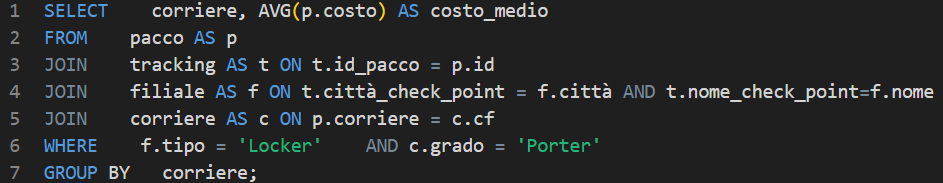
\includegraphics[width=1 \textwidth]{Resources/QUERY1.png}
\label{ML}
\end{figure}
2. \textbf{QUERY 2} Numero pacchi per bundle con garanzia 3 anni
\begin{figure}[H]
\centering
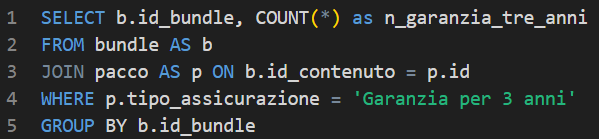
\includegraphics[width=1 \textwidth]{Resources/QUERY2.png}
\label{ML}
\end{figure}
3. \textbf{QUERY 3} Clienti con più di 2 pacchi consegnati per filiale
\begin{figure}[H]
\centering
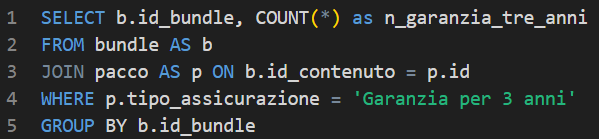
\includegraphics[width=1 \textwidth]{Resources/QUERY2.png}
\label{ML}
\end{figure}
4. \textbf{QUERY 4} Corrieri con bundle con pacchi con garanzia a 3 anni e costo maggiore di 300
\begin{figure}[H]
\centering
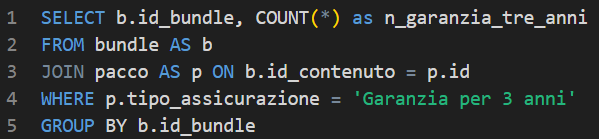
\includegraphics[width=1 \textwidth]{Resources/QUERY2.png}
\label{ML}
\end{figure} 
5. \textbf{QUERY 5} Ultimo aggiornamento del tracking di un pacco
\begin{figure}[H]
\centering
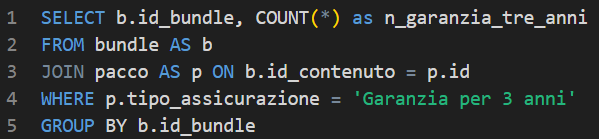
\includegraphics[width=1 \textwidth]{Resources/QUERY2.png}
\label{ML}
\end{figure}

\subsection{Creazione degli Indici} 

Supponendo di voler ottimizzare la query num 5, si deve considerare:

\begin{itemize}
  \item Condizione del JOIN: \texttt{p.cliente = c.email}
  \item Condizione del JOIN: \texttt{p.id = t.id\_pacco}
  \item Condizione del JOIN: \texttt{t.città\_check\_point = f.città AND t.nome\_check\_point = f.nome}
  \item Condizione del WHERE: \texttt{t.status = 'Consegnato'}
  \item GROUP BY sulle colonne: \texttt{c.email}, \texttt{f.nome}, \texttt{f.città}
  \item HAVING sulla funzione di aggregazione 
\end{itemize}


\noindent Per il punto 1 è opportuno creare due indici hash su entrambe le colonne del join:
\begin{figure}[H]
\centering
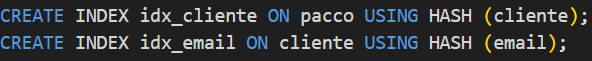
\includegraphics[width=1 \textwidth]{Resources/INDEX1.png}
\label{ML}
\end{figure}

\noindent Per il punto 2 è opportuno creare due indici hash su entrambe le colonne del join:
\begin{figure}[H]
\centering
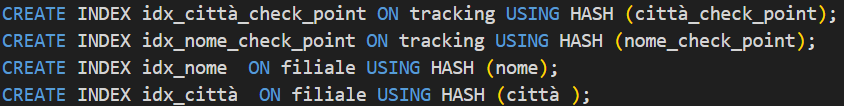
\includegraphics[width=1 \textwidth]{Resources/INDEX2.png}
\label{ML}
\end{figure}

\noindent Per il punto 3 è opportuno creare 4 indici hash su per tutte le condizioni del join:

\begin{figure}[H]
\centering
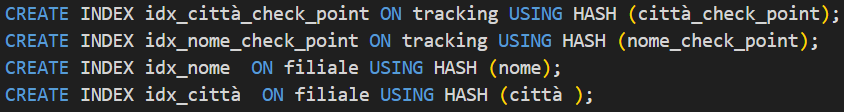
\includegraphics[width=1 \textwidth]{Resources/INDEX3.png}
\label{ML}
\end{figure}

\noindent Per il punto 4 è opportuno creare un indice sull'attributo rispetto a cui il WHERE valuta la sua condizione:

\begin{figure}[H]
\centering
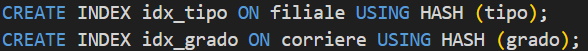
\includegraphics[width=1 \textwidth]{Resources/INDEX4.png}
\label{ML}
\end{figure}

\noindent Il punto 6 è un GROUP BY e potrebbe quindi essere ottimizzato tramite il seguente indice B+Tree:

\begin{figure}[H]
\centering
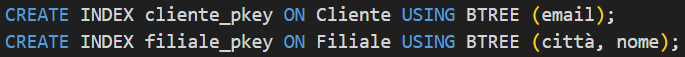
\includegraphics[width=1 \textwidth]{Resources/INDEX5.png}
\label{ML}
\end{figure}  

\noindent Nella pratica, non è necessario tuttavia creare tale indice perché, come anche altri
sistemi, PostgreSQL automaticamente crea un indice B+ Tree per ogni chiave primaria; in particolare, quindi, esiste già un indice B+Tree per FILIALE e per CLIENTE.
\noindent Effettivamente, provando a creare i sudetti indici si ottiene un errore che riporta che sono già esistenti.